% Options for packages loaded elsewhere
% Options for packages loaded elsewhere
\PassOptionsToPackage{unicode}{hyperref}
\PassOptionsToPackage{hyphens}{url}
\PassOptionsToPackage{dvipsnames,svgnames,x11names}{xcolor}
%
\documentclass[
]{article}
\usepackage{xcolor}
\usepackage{amsmath,amssymb}
\setcounter{secnumdepth}{5}
\usepackage{iftex}
\ifPDFTeX
  \usepackage[T1]{fontenc}
  \usepackage[utf8]{inputenc}
  \usepackage{textcomp} % provide euro and other symbols
\else % if luatex or xetex
  \usepackage{unicode-math} % this also loads fontspec
  \defaultfontfeatures{Scale=MatchLowercase}
  \defaultfontfeatures[\rmfamily]{Ligatures=TeX,Scale=1}
\fi
\usepackage{lmodern}
\ifPDFTeX\else
  % xetex/luatex font selection
\fi
% Use upquote if available, for straight quotes in verbatim environments
\IfFileExists{upquote.sty}{\usepackage{upquote}}{}
\IfFileExists{microtype.sty}{% use microtype if available
  \usepackage[]{microtype}
  \UseMicrotypeSet[protrusion]{basicmath} % disable protrusion for tt fonts
}{}
\makeatletter
\@ifundefined{KOMAClassName}{% if non-KOMA class
  \IfFileExists{parskip.sty}{%
    \usepackage{parskip}
  }{% else
    \setlength{\parindent}{0pt}
    \setlength{\parskip}{6pt plus 2pt minus 1pt}}
}{% if KOMA class
  \KOMAoptions{parskip=half}}
\makeatother
% Make \paragraph and \subparagraph free-standing
\makeatletter
\ifx\paragraph\undefined\else
  \let\oldparagraph\paragraph
  \renewcommand{\paragraph}{
    \@ifstar
      \xxxParagraphStar
      \xxxParagraphNoStar
  }
  \newcommand{\xxxParagraphStar}[1]{\oldparagraph*{#1}\mbox{}}
  \newcommand{\xxxParagraphNoStar}[1]{\oldparagraph{#1}\mbox{}}
\fi
\ifx\subparagraph\undefined\else
  \let\oldsubparagraph\subparagraph
  \renewcommand{\subparagraph}{
    \@ifstar
      \xxxSubParagraphStar
      \xxxSubParagraphNoStar
  }
  \newcommand{\xxxSubParagraphStar}[1]{\oldsubparagraph*{#1}\mbox{}}
  \newcommand{\xxxSubParagraphNoStar}[1]{\oldsubparagraph{#1}\mbox{}}
\fi
\makeatother

\usepackage{color}
\usepackage{fancyvrb}
\newcommand{\VerbBar}{|}
\newcommand{\VERB}{\Verb[commandchars=\\\{\}]}
\DefineVerbatimEnvironment{Highlighting}{Verbatim}{commandchars=\\\{\}}
% Add ',fontsize=\small' for more characters per line
\usepackage{framed}
\definecolor{shadecolor}{RGB}{241,243,245}
\newenvironment{Shaded}{\begin{snugshade}}{\end{snugshade}}
\newcommand{\AlertTok}[1]{\textcolor[rgb]{0.68,0.00,0.00}{#1}}
\newcommand{\AnnotationTok}[1]{\textcolor[rgb]{0.37,0.37,0.37}{#1}}
\newcommand{\AttributeTok}[1]{\textcolor[rgb]{0.40,0.45,0.13}{#1}}
\newcommand{\BaseNTok}[1]{\textcolor[rgb]{0.68,0.00,0.00}{#1}}
\newcommand{\BuiltInTok}[1]{\textcolor[rgb]{0.00,0.23,0.31}{#1}}
\newcommand{\CharTok}[1]{\textcolor[rgb]{0.13,0.47,0.30}{#1}}
\newcommand{\CommentTok}[1]{\textcolor[rgb]{0.37,0.37,0.37}{#1}}
\newcommand{\CommentVarTok}[1]{\textcolor[rgb]{0.37,0.37,0.37}{\textit{#1}}}
\newcommand{\ConstantTok}[1]{\textcolor[rgb]{0.56,0.35,0.01}{#1}}
\newcommand{\ControlFlowTok}[1]{\textcolor[rgb]{0.00,0.23,0.31}{\textbf{#1}}}
\newcommand{\DataTypeTok}[1]{\textcolor[rgb]{0.68,0.00,0.00}{#1}}
\newcommand{\DecValTok}[1]{\textcolor[rgb]{0.68,0.00,0.00}{#1}}
\newcommand{\DocumentationTok}[1]{\textcolor[rgb]{0.37,0.37,0.37}{\textit{#1}}}
\newcommand{\ErrorTok}[1]{\textcolor[rgb]{0.68,0.00,0.00}{#1}}
\newcommand{\ExtensionTok}[1]{\textcolor[rgb]{0.00,0.23,0.31}{#1}}
\newcommand{\FloatTok}[1]{\textcolor[rgb]{0.68,0.00,0.00}{#1}}
\newcommand{\FunctionTok}[1]{\textcolor[rgb]{0.28,0.35,0.67}{#1}}
\newcommand{\ImportTok}[1]{\textcolor[rgb]{0.00,0.46,0.62}{#1}}
\newcommand{\InformationTok}[1]{\textcolor[rgb]{0.37,0.37,0.37}{#1}}
\newcommand{\KeywordTok}[1]{\textcolor[rgb]{0.00,0.23,0.31}{\textbf{#1}}}
\newcommand{\NormalTok}[1]{\textcolor[rgb]{0.00,0.23,0.31}{#1}}
\newcommand{\OperatorTok}[1]{\textcolor[rgb]{0.37,0.37,0.37}{#1}}
\newcommand{\OtherTok}[1]{\textcolor[rgb]{0.00,0.23,0.31}{#1}}
\newcommand{\PreprocessorTok}[1]{\textcolor[rgb]{0.68,0.00,0.00}{#1}}
\newcommand{\RegionMarkerTok}[1]{\textcolor[rgb]{0.00,0.23,0.31}{#1}}
\newcommand{\SpecialCharTok}[1]{\textcolor[rgb]{0.37,0.37,0.37}{#1}}
\newcommand{\SpecialStringTok}[1]{\textcolor[rgb]{0.13,0.47,0.30}{#1}}
\newcommand{\StringTok}[1]{\textcolor[rgb]{0.13,0.47,0.30}{#1}}
\newcommand{\VariableTok}[1]{\textcolor[rgb]{0.07,0.07,0.07}{#1}}
\newcommand{\VerbatimStringTok}[1]{\textcolor[rgb]{0.13,0.47,0.30}{#1}}
\newcommand{\WarningTok}[1]{\textcolor[rgb]{0.37,0.37,0.37}{\textit{#1}}}

\usepackage{longtable,booktabs,array}
\usepackage{calc} % for calculating minipage widths
% Correct order of tables after \paragraph or \subparagraph
\usepackage{etoolbox}
\makeatletter
\patchcmd\longtable{\par}{\if@noskipsec\mbox{}\fi\par}{}{}
\makeatother
% Allow footnotes in longtable head/foot
\IfFileExists{footnotehyper.sty}{\usepackage{footnotehyper}}{\usepackage{footnote}}
\makesavenoteenv{longtable}
\usepackage{graphicx}
\makeatletter
\newsavebox\pandoc@box
\newcommand*\pandocbounded[1]{% scales image to fit in text height/width
  \sbox\pandoc@box{#1}%
  \Gscale@div\@tempa{\textheight}{\dimexpr\ht\pandoc@box+\dp\pandoc@box\relax}%
  \Gscale@div\@tempb{\linewidth}{\wd\pandoc@box}%
  \ifdim\@tempb\p@<\@tempa\p@\let\@tempa\@tempb\fi% select the smaller of both
  \ifdim\@tempa\p@<\p@\scalebox{\@tempa}{\usebox\pandoc@box}%
  \else\usebox{\pandoc@box}%
  \fi%
}
% Set default figure placement to htbp
\def\fps@figure{htbp}
\makeatother


% definitions for citeproc citations
\NewDocumentCommand\citeproctext{}{}
\NewDocumentCommand\citeproc{mm}{%
  \begingroup\def\citeproctext{#2}\cite{#1}\endgroup}
\makeatletter
 % allow citations to break across lines
 \let\@cite@ofmt\@firstofone
 % avoid brackets around text for \cite:
 \def\@biblabel#1{}
 \def\@cite#1#2{{#1\if@tempswa , #2\fi}}
\makeatother
\newlength{\cslhangindent}
\setlength{\cslhangindent}{1.5em}
\newlength{\csllabelwidth}
\setlength{\csllabelwidth}{3em}
\newenvironment{CSLReferences}[2] % #1 hanging-indent, #2 entry-spacing
 {\begin{list}{}{%
  \setlength{\itemindent}{0pt}
  \setlength{\leftmargin}{0pt}
  \setlength{\parsep}{0pt}
  % turn on hanging indent if param 1 is 1
  \ifodd #1
   \setlength{\leftmargin}{\cslhangindent}
   \setlength{\itemindent}{-1\cslhangindent}
  \fi
  % set entry spacing
  \setlength{\itemsep}{#2\baselineskip}}}
 {\end{list}}
\usepackage{calc}
\newcommand{\CSLBlock}[1]{\hfill\break\parbox[t]{\linewidth}{\strut\ignorespaces#1\strut}}
\newcommand{\CSLLeftMargin}[1]{\parbox[t]{\csllabelwidth}{\strut#1\strut}}
\newcommand{\CSLRightInline}[1]{\parbox[t]{\linewidth - \csllabelwidth}{\strut#1\strut}}
\newcommand{\CSLIndent}[1]{\hspace{\cslhangindent}#1}



\setlength{\emergencystretch}{3em} % prevent overfull lines

\providecommand{\tightlist}{%
  \setlength{\itemsep}{0pt}\setlength{\parskip}{0pt}}



 


\makeatletter
\@ifpackageloaded{tcolorbox}{}{\usepackage[skins,breakable]{tcolorbox}}
\@ifpackageloaded{fontawesome5}{}{\usepackage{fontawesome5}}
\definecolor{quarto-callout-color}{HTML}{909090}
\definecolor{quarto-callout-note-color}{HTML}{0758E5}
\definecolor{quarto-callout-important-color}{HTML}{CC1914}
\definecolor{quarto-callout-warning-color}{HTML}{EB9113}
\definecolor{quarto-callout-tip-color}{HTML}{00A047}
\definecolor{quarto-callout-caution-color}{HTML}{FC5300}
\definecolor{quarto-callout-color-frame}{HTML}{acacac}
\definecolor{quarto-callout-note-color-frame}{HTML}{4582ec}
\definecolor{quarto-callout-important-color-frame}{HTML}{d9534f}
\definecolor{quarto-callout-warning-color-frame}{HTML}{f0ad4e}
\definecolor{quarto-callout-tip-color-frame}{HTML}{02b875}
\definecolor{quarto-callout-caution-color-frame}{HTML}{fd7e14}
\makeatother
\makeatletter
\@ifpackageloaded{caption}{}{\usepackage{caption}}
\AtBeginDocument{%
\ifdefined\contentsname
  \renewcommand*\contentsname{Table of contents}
\else
  \newcommand\contentsname{Table of contents}
\fi
\ifdefined\listfigurename
  \renewcommand*\listfigurename{List of Figures}
\else
  \newcommand\listfigurename{List of Figures}
\fi
\ifdefined\listtablename
  \renewcommand*\listtablename{List of Tables}
\else
  \newcommand\listtablename{List of Tables}
\fi
\ifdefined\figurename
  \renewcommand*\figurename{Figure}
\else
  \newcommand\figurename{Figure}
\fi
\ifdefined\tablename
  \renewcommand*\tablename{Table}
\else
  \newcommand\tablename{Table}
\fi
}
\@ifpackageloaded{float}{}{\usepackage{float}}
\floatstyle{ruled}
\@ifundefined{c@chapter}{\newfloat{codelisting}{h}{lop}}{\newfloat{codelisting}{h}{lop}[chapter]}
\floatname{codelisting}{Listing}
\newcommand*\listoflistings{\listof{codelisting}{List of Listings}}
\makeatother
\makeatletter
\makeatother
\makeatletter
\@ifpackageloaded{caption}{}{\usepackage{caption}}
\@ifpackageloaded{subcaption}{}{\usepackage{subcaption}}
\makeatother
\usepackage{bookmark}
\IfFileExists{xurl.sty}{\usepackage{xurl}}{} % add URL line breaks if available
\urlstyle{same}
\hypersetup{
  pdftitle={Análisis de Supervivencia},
  pdfauthor={Sergio M. Nava Muñoz},
  colorlinks=true,
  linkcolor={blue},
  filecolor={Maroon},
  citecolor={Blue},
  urlcolor={Blue},
  pdfcreator={LaTeX via pandoc}}


\title{Análisis de Supervivencia}
\usepackage{etoolbox}
\makeatletter
\providecommand{\subtitle}[1]{% add subtitle to \maketitle
  \apptocmd{\@title}{\par {\large #1 \par}}{}{}
}
\makeatother
\subtitle{Modelo de Riesgos Proporcionales de Cox}
\author{Sergio M. Nava Muñoz}
\date{2025-06-01}
\begin{document}
\maketitle

\renewcommand*\contentsname{Table of contents}
{
\hypersetup{linkcolor=}
\setcounter{tocdepth}{2}
\tableofcontents
}

\section{Introducción}\label{introducciuxf3n}

\begin{itemize}
\tightlist
\item
  El modelo de riesgos proporcionales de Cox es el más utilizado para
  analizar datos de supervivencia con múltiples covariables.
\item
  Modelo de regresión \textbf{semiparamétrico}.
\item
  Basado en Klein \& Moeschberger (2003).
\end{itemize}

\begin{center}\rule{0.5\linewidth}{0.5pt}\end{center}

\section{Fundamento Matemático del
Modelo}\label{fundamento-matemuxe1tico-del-modelo}

\[
h(t|X) = h_0(t) \cdot \exp(\beta^T X)
\]

\begin{itemize}
\tightlist
\item
  \(h(t|X)\): función de riesgo condicional.
\item
  \(h_0(t)\): riesgo base (no especificado).
\item
  \(X\): vector de covariables.
\item
  \(\beta\): coeficientes a estimar.
\end{itemize}

\begin{center}\rule{0.5\linewidth}{0.5pt}\end{center}

\section{Suposición de Riesgos Proporcionales
(PH)}\label{suposiciuxf3n-de-riesgos-proporcionales-ph}

\begin{itemize}
\item
  La razón de riesgos entre dos individuos: \[
  \frac{h(t|X_1)}{h(t|X_2)} = \exp(\beta^T(X_1 - X_2))
  \] compara el riesgo de dos individuos con distintos valores de
  covariables \(X_1\) y \(X_2\), en el mismo tiempo \(t\).
\item
  No depende del tiempo → \textbf{proporcionalidad}.
\item
  Si las funciones de riesgo se cruzan, la suposición PH se viola.
\end{itemize}

\subsection{Ejemplo concreto}\label{ejemplo-concreto}

Supongamos un modelo con dos covariables:

\begin{itemize}
\tightlist
\item
  \texttt{tratamiento}: 0 = control, 1 = experimental
\item
  \texttt{edad}: en años
\end{itemize}

Y los coeficientes estimados son:

\begin{itemize}
\tightlist
\item
  \(\beta = (-0.5, 0.04)\)
\end{itemize}

\begin{Shaded}
\begin{Highlighting}[]
\CommentTok{\# Vectores de covariables para dos individuos}
\NormalTok{X1 }\OtherTok{\textless{}{-}} \FunctionTok{c}\NormalTok{(}\AttributeTok{tratamiento =} \DecValTok{1}\NormalTok{, }\AttributeTok{edad =} \DecValTok{60}\NormalTok{)}
\NormalTok{X2 }\OtherTok{\textless{}{-}} \FunctionTok{c}\NormalTok{(}\AttributeTok{tratamiento =} \DecValTok{0}\NormalTok{, }\AttributeTok{edad =} \DecValTok{60}\NormalTok{)}

\CommentTok{\# Coeficientes estimados del modelo}
\NormalTok{beta }\OtherTok{\textless{}{-}} \FunctionTok{c}\NormalTok{(}\SpecialCharTok{{-}}\FloatTok{0.5}\NormalTok{, }\FloatTok{0.04}\NormalTok{)}

\CommentTok{\# Cálculo de la razón de riesgos}
\NormalTok{HR }\OtherTok{\textless{}{-}} \FunctionTok{exp}\NormalTok{(}\FunctionTok{sum}\NormalTok{(beta }\SpecialCharTok{*}\NormalTok{ (X1 }\SpecialCharTok{{-}}\NormalTok{ X2)))}
\NormalTok{HR}
\end{Highlighting}
\end{Shaded}

\begin{verbatim}
[1] 0.6065307
\end{verbatim}

\begin{center}\rule{0.5\linewidth}{0.5pt}\end{center}

\subsection{Ejemplo cuando no se cumple la
proporcionalidad}\label{ejemplo-cuando-no-se-cumple-la-proporcionalidad}

\begin{Shaded}
\begin{Highlighting}[]
\FunctionTok{library}\NormalTok{(survival)}
\FunctionTok{library}\NormalTok{(survminer)}

\CommentTok{\# Cargar datos}
\FunctionTok{data}\NormalTok{(lung)}

\CommentTok{\# Re{-}codificar status: 2 = evento, 1 = censura → convertir a 1/0}
\NormalTok{lung}\SpecialCharTok{$}\NormalTok{status2 }\OtherTok{\textless{}{-}} \FunctionTok{ifelse}\NormalTok{(lung}\SpecialCharTok{$}\NormalTok{status }\SpecialCharTok{==} \DecValTok{2}\NormalTok{, }\DecValTok{1}\NormalTok{, }\DecValTok{0}\NormalTok{)}

\CommentTok{\# Verificar niveles de sexo}
\FunctionTok{table}\NormalTok{(lung}\SpecialCharTok{$}\NormalTok{sex)  }\CommentTok{\# 1 = hombre, 2 = mujer}
\end{Highlighting}
\end{Shaded}

\begin{verbatim}

  1   2 
138  90 
\end{verbatim}

\begin{Shaded}
\begin{Highlighting}[]
\NormalTok{fit\_km }\OtherTok{\textless{}{-}} \FunctionTok{survfit}\NormalTok{(}\FunctionTok{Surv}\NormalTok{(time, status2) }\SpecialCharTok{\textasciitilde{}} \FunctionTok{factor}\NormalTok{(sex), }\AttributeTok{data =}\NormalTok{ lung)}

\FunctionTok{ggsurvplot}\NormalTok{(fit\_km,}
           \AttributeTok{data =}\NormalTok{ lung,}
           \AttributeTok{conf.int =} \ConstantTok{TRUE}\NormalTok{,}
           \AttributeTok{legend.labs =} \FunctionTok{c}\NormalTok{(}\StringTok{"Hombre"}\NormalTok{, }\StringTok{"Mujer"}\NormalTok{),}
           \AttributeTok{xlab =} \StringTok{"Días"}\NormalTok{, }\AttributeTok{ylab =} \StringTok{"Supervivencia estimada"}\NormalTok{,}
           \AttributeTok{title =} \StringTok{"Curvas Kaplan{-}Meier por sexo"}\NormalTok{)}
\end{Highlighting}
\end{Shaded}

\pandocbounded{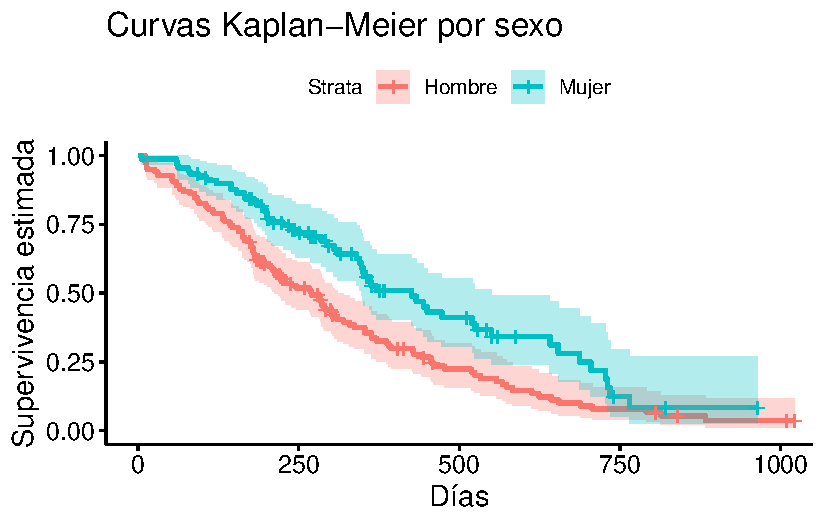
\includegraphics[keepaspectratio]{Unidad4_files/figure-pdf/unnamed-chunk-4-1.pdf}}

\begin{quote}
Si las curvas se cruzan, puede indicar que la suposición de riesgos
proporcionales se viola.
\end{quote}

\begin{center}\rule{0.5\linewidth}{0.5pt}\end{center}

\section{Características del
Modelo}\label{caracteruxedsticas-del-modelo}

\begin{itemize}
\tightlist
\item
  \textbf{Semiparamétrico}: no se asume forma para \(h_0(t)\).
\item
  Estimación de coeficientes mediante \textbf{verosimilitud parcial}.
\item
  Robusto y flexible ante diferentes tipos de datos censurados.
\end{itemize}

\begin{center}\rule{0.5\linewidth}{0.5pt}\end{center}

\section{Interpretación de los
coeficientes}\label{interpretaciuxf3n-de-los-coeficientes}

\subsection{Razón de Riesgo (HR)}\label{razuxf3n-de-riesgo-hr}

\begin{itemize}
\tightlist
\item
  \(HR = \exp(\beta)\).
\item
  HR \textgreater{} 1: mayor riesgo.
\item
  HR \textless{} 1: efecto protector.
\item
  HR ≈ 1 : no afecta el riesgo.
\end{itemize}

\subsection{Ejemplos de interpretación de
HR}\label{ejemplos-de-interpretaciuxf3n-de-hr}

\begin{longtable}[]{@{}
  >{\raggedright\arraybackslash}p{(\linewidth - 6\tabcolsep) * \real{0.4000}}
  >{\raggedleft\arraybackslash}p{(\linewidth - 6\tabcolsep) * \real{0.1263}}
  >{\raggedleft\arraybackslash}p{(\linewidth - 6\tabcolsep) * \real{0.0632}}
  >{\raggedright\arraybackslash}p{(\linewidth - 6\tabcolsep) * \real{0.4105}}@{}}
\caption{Ejemplos de interpretación de razones de riesgo
(HR)}\tabularnewline
\toprule\noalign{}
\begin{minipage}[b]{\linewidth}\raggedright
Variable
\end{minipage} & \begin{minipage}[b]{\linewidth}\raggedleft
Coeficiente
\end{minipage} & \begin{minipage}[b]{\linewidth}\raggedleft
HR
\end{minipage} & \begin{minipage}[b]{\linewidth}\raggedright
Interpretación
\end{minipage} \\
\midrule\noalign{}
\endfirsthead
\toprule\noalign{}
\begin{minipage}[b]{\linewidth}\raggedright
Variable
\end{minipage} & \begin{minipage}[b]{\linewidth}\raggedleft
Coeficiente
\end{minipage} & \begin{minipage}[b]{\linewidth}\raggedleft
HR
\end{minipage} & \begin{minipage}[b]{\linewidth}\raggedright
Interpretación
\end{minipage} \\
\midrule\noalign{}
\endhead
\bottomrule\noalign{}
\endlastfoot
tratamiento (experimental vs control) & -0.510 & 0.600 & 40\% menos
riesgo en grupo experimental \\
edad (años) & 0.050 & 1.051 & Cada año adicional → +5.1\% riesgo \\
karno (índice Karnofsky) & -0.032 & 0.969 & Cada punto adicional →
-3.2\% riesgo \\
\end{longtable}

\begin{center}\rule{0.5\linewidth}{0.5pt}\end{center}

\section{Ejemplo computacional: Modelo de Cox
PH}\label{ejemplo-computacional-modelo-de-cox-ph}

Analizaremos el modelo de Cox PH usando una base de datos de remisión en
pacientes con leucemia (Freireich et al. (1963)).

\begin{itemize}
\tightlist
\item
  Dos grupos con 21 pacientes cada uno:\textbf{Grupo 1} (Tratamiento),
  \textbf{Grupo 2} (Placebo)
\item
  Covariable adicional: \textbf{log WBC}, un importante predictor
  pronóstico en leucemia.
\end{itemize}

\textbf{Pregunta de investigación}: Comparar la supervivencia entre
grupos, \textbf{ajustando por posibles efectos de confusión o
interacción con log WBC}.

\begin{tcolorbox}[enhanced jigsaw, rightrule=.15mm, toprule=.15mm, leftrule=.75mm, opacityback=0, left=2mm, colback=white, colframe=quarto-callout-note-color-frame, arc=.35mm, bottomrule=.15mm, breakable]

\begin{longtable}[]{@{}cccc@{}}
\caption{Leukemia Remission Data: Group 1 (Treatment) vs Group 2
(Placebo)}\tabularnewline
\toprule\noalign{}
t.Grupo.1. & log.WBC..Grupo.1. & t.Grupo.2. & log.WBC..Grupo.2. \\
\midrule\noalign{}
\endfirsthead
\toprule\noalign{}
t.Grupo.1. & log.WBC..Grupo.1. & t.Grupo.2. & log.WBC..Grupo.2. \\
\midrule\noalign{}
\endhead
\bottomrule\noalign{}
\endlastfoot
6 & 2.31 & 1 & 2.80 \\
6 & 4.06 & 1 & 5.00 \\
6 & 3.28 & 2 & 4.91 \\
7 & 4.43 & 2 & 4.48 \\
10 & 2.96 & 3 & 4.01 \\
13 & 2.88 & 4 & 4.36 \\
16 & 3.60 & 4 & 2.42 \\
22 & 2.32 & 5 & 3.49 \\
23 & 2.57 & 5 & 3.97 \\
6+ & 3.20 & 8 & 3.52 \\
9+ & 2.80 & 8 & 3.05 \\
10+ & 2.70 & 8 & 2.32 \\
11+ & 2.60 & 8 & 3.26 \\
17+ & 2.16 & 11 & 3.49 \\
19+ & 2.05 & 11 & 2.12 \\
20+ & 2.01 & 12 & 1.50 \\
25+ & 1.78 & 12 & 3.06 \\
32+ & 2.20 & 15 & 2.30 \\
32+ & 2.53 & 17 & 2.95 \\
34+ & 1.47 & 22 & 2.73 \\
35+ & 1.45 & 23 & 1.97 \\
\end{longtable}

\end{tcolorbox}

\begin{center}\rule{0.5\linewidth}{0.5pt}\end{center}

\subsection{Datos de Leucemia}\label{datos-de-leucemia}

\begin{Shaded}
\begin{Highlighting}[]
\NormalTok{leukemia }\OtherTok{\textless{}{-}} \FunctionTok{data.frame}\NormalTok{(}
  \AttributeTok{time =} \FunctionTok{c}\NormalTok{(}\DecValTok{6}\NormalTok{, }\DecValTok{6}\NormalTok{, }\DecValTok{6}\NormalTok{, }\DecValTok{7}\NormalTok{, }\DecValTok{10}\NormalTok{, }\DecValTok{13}\NormalTok{, }\DecValTok{16}\NormalTok{, }\DecValTok{22}\NormalTok{, }\DecValTok{23}\NormalTok{, }\DecValTok{6}\NormalTok{, }\DecValTok{9}\NormalTok{, }\DecValTok{10}\NormalTok{, }\DecValTok{11}\NormalTok{, }\DecValTok{17}\NormalTok{, }\DecValTok{19}\NormalTok{, }\DecValTok{20}\NormalTok{, }\DecValTok{25}\NormalTok{, }\DecValTok{32}\NormalTok{, }\DecValTok{32}\NormalTok{, }\DecValTok{34}\NormalTok{, }\DecValTok{35}\NormalTok{,}
           \DecValTok{1}\NormalTok{, }\DecValTok{1}\NormalTok{, }\DecValTok{2}\NormalTok{, }\DecValTok{2}\NormalTok{, }\DecValTok{3}\NormalTok{, }\DecValTok{4}\NormalTok{, }\DecValTok{4}\NormalTok{, }\DecValTok{5}\NormalTok{, }\DecValTok{5}\NormalTok{, }\DecValTok{8}\NormalTok{, }\DecValTok{8}\NormalTok{, }\DecValTok{8}\NormalTok{, }\DecValTok{8}\NormalTok{, }\DecValTok{11}\NormalTok{, }\DecValTok{11}\NormalTok{, }\DecValTok{12}\NormalTok{, }\DecValTok{12}\NormalTok{, }\DecValTok{15}\NormalTok{, }\DecValTok{17}\NormalTok{, }\DecValTok{22}\NormalTok{, }\DecValTok{23}\NormalTok{),}
  \AttributeTok{status =} \FunctionTok{c}\NormalTok{(}\FunctionTok{rep}\NormalTok{(}\DecValTok{1}\NormalTok{, }\DecValTok{9}\NormalTok{), }\FunctionTok{rep}\NormalTok{(}\DecValTok{0}\NormalTok{, }\DecValTok{12}\NormalTok{), }\FunctionTok{rep}\NormalTok{(}\DecValTok{1}\NormalTok{, }\DecValTok{21}\NormalTok{)),}
  \AttributeTok{group =} \FunctionTok{c}\NormalTok{(}\FunctionTok{rep}\NormalTok{(}\DecValTok{1}\NormalTok{, }\DecValTok{21}\NormalTok{), }\FunctionTok{rep}\NormalTok{(}\DecValTok{2}\NormalTok{, }\DecValTok{21}\NormalTok{)),}
  \AttributeTok{logWBC =} \FunctionTok{c}\NormalTok{(}\FloatTok{2.31}\NormalTok{, }\FloatTok{4.06}\NormalTok{, }\FloatTok{3.28}\NormalTok{, }\FloatTok{4.43}\NormalTok{, }\FloatTok{2.96}\NormalTok{, }\FloatTok{2.88}\NormalTok{, }\FloatTok{3.60}\NormalTok{, }\FloatTok{2.32}\NormalTok{, }\FloatTok{2.57}\NormalTok{, }
             \FloatTok{3.20}\NormalTok{, }\FloatTok{2.80}\NormalTok{, }\FloatTok{2.70}\NormalTok{, }\FloatTok{2.60}\NormalTok{, }\FloatTok{2.16}\NormalTok{, }\FloatTok{2.05}\NormalTok{, }\FloatTok{2.01}\NormalTok{, }\FloatTok{1.78}\NormalTok{, }\FloatTok{2.20}\NormalTok{, }\FloatTok{2.53}\NormalTok{, }\FloatTok{1.47}\NormalTok{, }\FloatTok{1.45}\NormalTok{,}
             \FloatTok{2.80}\NormalTok{, }\FloatTok{5.00}\NormalTok{, }\FloatTok{4.91}\NormalTok{, }\FloatTok{4.48}\NormalTok{, }\FloatTok{4.01}\NormalTok{, }\FloatTok{4.36}\NormalTok{, }\FloatTok{2.42}\NormalTok{, }\FloatTok{3.49}\NormalTok{, }\FloatTok{3.97}\NormalTok{, }
             \FloatTok{3.52}\NormalTok{, }\FloatTok{3.05}\NormalTok{, }\FloatTok{2.32}\NormalTok{, }\FloatTok{3.26}\NormalTok{, }\FloatTok{3.49}\NormalTok{, }\FloatTok{2.12}\NormalTok{, }\FloatTok{1.50}\NormalTok{, }\FloatTok{3.06}\NormalTok{, }\FloatTok{2.30}\NormalTok{, }\FloatTok{2.95}\NormalTok{, }\FloatTok{2.73}\NormalTok{, }\FloatTok{1.97}\NormalTok{)}
\NormalTok{)}
\end{Highlighting}
\end{Shaded}

\textbf{Explicación}: Este conjunto representa a pacientes con leucemia,
donde \texttt{time} es el tiempo hasta recaída (o censura),
\texttt{status} indica si ocurrió el evento (1) o no (0), \texttt{group}
es el tratamiento (1 = tratado, 2 = placebo) y \texttt{logWBC} es el
logaritmo del conteo de glóbulos blancos.

\begin{Shaded}
\begin{Highlighting}[]
\FunctionTok{summary}\NormalTok{(leukemia)}
\end{Highlighting}
\end{Shaded}

\begin{verbatim}
      time           status           group         logWBC     
 Min.   : 1.00   Min.   :0.0000   Min.   :1.0   Min.   :1.450  
 1st Qu.: 6.00   1st Qu.:0.0000   1st Qu.:1.0   1st Qu.:2.303  
 Median :10.50   Median :1.0000   Median :1.5   Median :2.800  
 Mean   :12.88   Mean   :0.7143   Mean   :1.5   Mean   :2.930  
 3rd Qu.:18.50   3rd Qu.:1.0000   3rd Qu.:2.0   3rd Qu.:3.490  
 Max.   :35.00   Max.   :1.0000   Max.   :2.0   Max.   :5.000  
\end{verbatim}

\begin{Shaded}
\begin{Highlighting}[]
\FunctionTok{table}\NormalTok{(leukemia}\SpecialCharTok{$}\NormalTok{status,leukemia}\SpecialCharTok{$}\NormalTok{group)}
\end{Highlighting}
\end{Shaded}

\begin{verbatim}
   
     1  2
  0 12  0
  1  9 21
\end{verbatim}

\begin{center}\rule{0.5\linewidth}{0.5pt}\end{center}

\begin{Shaded}
\begin{Highlighting}[]
\NormalTok{fit }\OtherTok{\textless{}{-}} \FunctionTok{survfit}\NormalTok{(}\FunctionTok{Surv}\NormalTok{(time, status) }\SpecialCharTok{\textasciitilde{}}\NormalTok{ group, }\AttributeTok{data =}\NormalTok{ leukemia)}
\FunctionTok{ggsurvplot}\NormalTok{(fit, }\AttributeTok{xlab =} \StringTok{"Tiempo"}\NormalTok{, }\AttributeTok{ylab =} \StringTok{"Probabilidad de Supervivencia"}\NormalTok{)}
\end{Highlighting}
\end{Shaded}

\pandocbounded{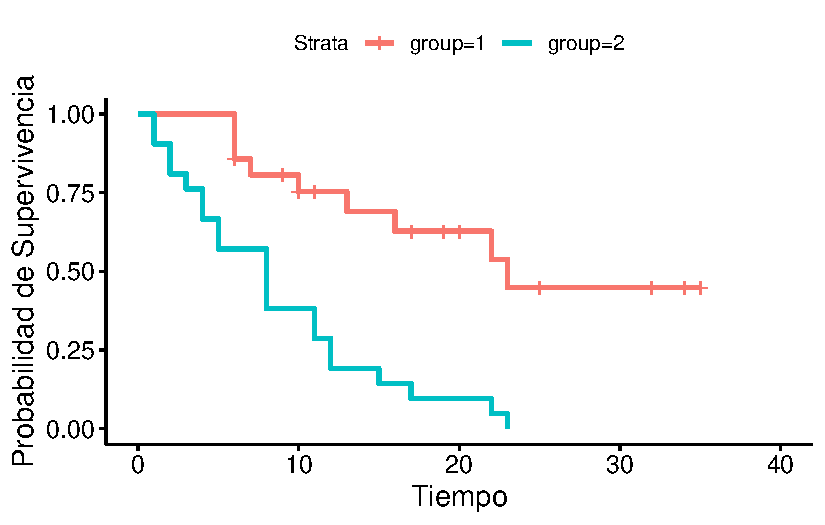
\includegraphics[keepaspectratio]{Unidad4_files/figure-pdf/unnamed-chunk-9-1.pdf}}

\begin{center}\rule{0.5\linewidth}{0.5pt}\end{center}

\begin{Shaded}
\begin{Highlighting}[]
\NormalTok{cox\_model }\OtherTok{\textless{}{-}} \FunctionTok{coxph}\NormalTok{(}\FunctionTok{Surv}\NormalTok{(time, status) }\SpecialCharTok{\textasciitilde{}} \FunctionTok{factor}\NormalTok{(group) }\SpecialCharTok{+}\NormalTok{ logWBC, }\AttributeTok{data =}\NormalTok{ leukemia)}
\FunctionTok{summary}\NormalTok{(cox\_model)}
\end{Highlighting}
\end{Shaded}

\begin{verbatim}
Call:
coxph(formula = Surv(time, status) ~ factor(group) + logWBC, 
    data = leukemia)

  n= 42, number of events= 30 

                 coef exp(coef) se(coef)     z Pr(>|z|)    
factor(group)2 1.3861    3.9991   0.4248 3.263   0.0011 ** 
logWBC         1.6909    5.4243   0.3359 5.034  4.8e-07 ***
---
Signif. codes:  0 '***' 0.001 '**' 0.01 '*' 0.05 '.' 0.1 ' ' 1

               exp(coef) exp(-coef) lower .95 upper .95
factor(group)2     3.999     0.2501     1.739     9.195
logWBC             5.424     0.1844     2.808    10.478

Concordance= 0.852  (se = 0.04 )
Likelihood ratio test= 46.71  on 2 df,   p=7e-11
Wald test            = 33.6  on 2 df,   p=5e-08
Score (logrank) test = 46.07  on 2 df,   p=1e-10
\end{verbatim}

\textbf{Explicación}: El modelo de Cox ajusta el riesgo de recaída según
el tratamiento y logWBC. \texttt{factor(group)} permite comparar placebo
contra tratamiento. La salida incluye coeficientes \texttt{beta},
errores estándar, valor z y p-valor.

\begin{center}\rule{0.5\linewidth}{0.5pt}\end{center}

\textbf{Interpretación del modelo (HR e IC)}

\begin{Shaded}
\begin{Highlighting}[]
\FunctionTok{exp}\NormalTok{(}\FunctionTok{coef}\NormalTok{(cox\_model))       }\CommentTok{\# Razón de riesgo (HR)}
\end{Highlighting}
\end{Shaded}

\begin{verbatim}
factor(group)2         logWBC 
      3.999125       5.424308 
\end{verbatim}

\begin{Shaded}
\begin{Highlighting}[]
\FunctionTok{exp}\NormalTok{(}\FunctionTok{confint}\NormalTok{(cox\_model))    }\CommentTok{\# Intervalo de confianza del 95\% para HR}
\end{Highlighting}
\end{Shaded}

\begin{verbatim}
                  2.5 %    97.5 %
factor(group)2 1.739306  9.195048
logWBC         2.808199 10.477578
\end{verbatim}

\textbf{Explicación}: Aquí se presentan los coeficientes exponenciados,
que se interpretan como razones de riesgo (HR). Un HR \textgreater{} 1
indica mayor riesgo relativo; HR \textless{} 1 sugiere efecto protector.
El intervalo de confianza permite evaluar si el efecto es
estadísticamente significativo (no debe incluir 1).

\begin{center}\rule{0.5\linewidth}{0.5pt}\end{center}

\textbf{Evaluación de la suposición de riesgos proporcionales}

\begin{Shaded}
\begin{Highlighting}[]
\NormalTok{test\_ph }\OtherTok{\textless{}{-}} \FunctionTok{cox.zph}\NormalTok{(cox\_model)}
\NormalTok{test\_ph}
\end{Highlighting}
\end{Shaded}

\begin{verbatim}
                 chisq df    p
factor(group) 8.27e-05  1 0.99
logWBC        4.00e-02  1 0.84
GLOBAL        4.02e-02  2 0.98
\end{verbatim}

\begin{Shaded}
\begin{Highlighting}[]
\FunctionTok{plot}\NormalTok{(test\_ph)}
\end{Highlighting}
\end{Shaded}

\pandocbounded{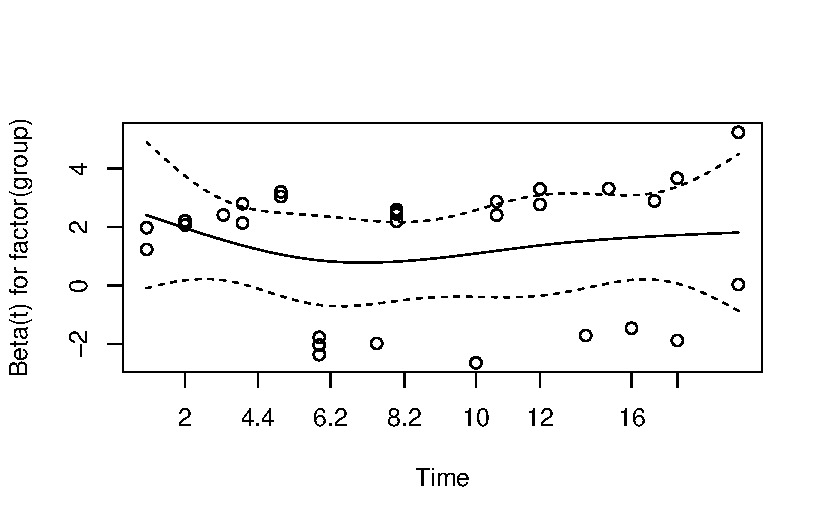
\includegraphics[keepaspectratio]{Unidad4_files/figure-pdf/unnamed-chunk-12-1.pdf}}

\pandocbounded{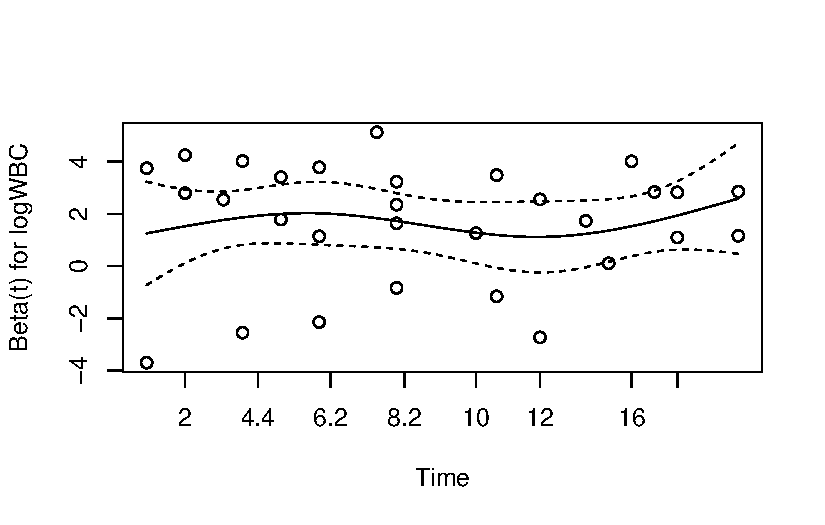
\includegraphics[keepaspectratio]{Unidad4_files/figure-pdf/unnamed-chunk-12-2.pdf}}

\begin{tcolorbox}[enhanced jigsaw, rightrule=.15mm, bottomrule=.15mm, left=2mm, arc=.35mm, colframe=quarto-callout-note-color-frame, title=\textcolor{quarto-callout-note-color}{\faInfo}\hspace{0.5em}{Hipótesis evaluadas con \texttt{cox.zph()}}, breakable, colbacktitle=quarto-callout-note-color!10!white, toprule=.15mm, coltitle=black, opacitybacktitle=0.6, leftrule=.75mm, opacityback=0, colback=white, titlerule=0mm, bottomtitle=1mm, toptitle=1mm]

\begin{itemize}
\tightlist
\item
  \textbf{Hipótesis nula (}\(H_0\)): la covariable cumple la suposición
  de riesgos proporcionales (el efecto de la covariable es constante en
  el tiempo).
\item
  \textbf{Hipótesis alternativa (}\(H_1\)): la covariable no cumple la
  suposición de riesgos proporcionales (el efecto cambia con el tiempo).
\end{itemize}

Un p-valor menor a 0.05 indica que se rechaza la hipótesis nula,
sugiriendo que la suposición de riesgos proporcionales \textbf{no se
cumple} para esa covariable.

El gráfico asociado muestra residuos de Schoenfeld.

\end{tcolorbox}

\begin{center}\rule{0.5\linewidth}{0.5pt}\end{center}

\subsection{Curvas de supervivencia
ajustadas}\label{curvas-de-supervivencia-ajustadas}

\pandocbounded{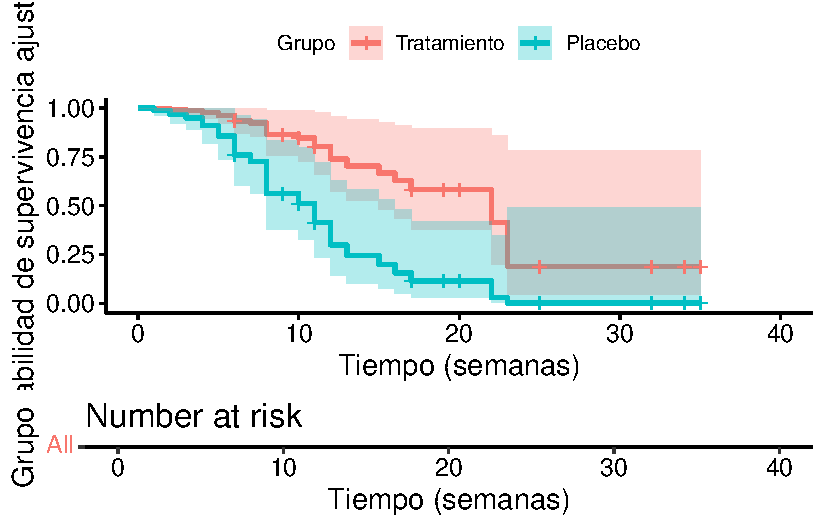
\includegraphics[keepaspectratio]{Unidad4_files/figure-pdf/unnamed-chunk-13-1.pdf}}

\textbf{Explicación}: Se grafican las curvas de supervivencia estimadas
para un paciente con nivel medio de logWBC, comparando tratamiento vs
placebo. El \texttt{risk.table} muestra cuántos pacientes permanecen en
riesgo a lo largo del tiempo.

\begin{center}\rule{0.5\linewidth}{0.5pt}\end{center}

\section{Evaluación de la Suposición
PH}\label{evaluaciuxf3n-de-la-suposiciuxf3n-ph}

\textbf{1. Gráficas}:

\begin{itemize}
\tightlist
\item
  Curvas log(-log) paralelas.
\item
  Gráficas de Schoenfeld residuals.
\end{itemize}

\textbf{2. Pruebas formales}:

\begin{itemize}
\tightlist
\item
  Test global de PH (e.g., \texttt{cox.zph} en R).
\end{itemize}

\textbf{3. Extensión con covariables dependientes del tiempo}:

\begin{itemize}
\tightlist
\item
  Incluir interacción con función del tiempo.
\end{itemize}

\begin{center}\rule{0.5\linewidth}{0.5pt}\end{center}

\subsection{Evaluación de proporcionalidad: Curvas
log(-log)}\label{evaluaciuxf3n-de-proporcionalidad-curvas-log-log}

\begin{itemize}
\tightlist
\item
  Otra forma gráfica de verificar la suposición de riesgos
  proporcionales.
\item
  Se grafican curvas:
\end{itemize}

\[
\log\{-\log[\hat{S}(t)]\}
\]

\begin{itemize}
\tightlist
\item
  Se esperan \textbf{curvas paralelas} si la suposición PH se cumple.
\item
  Se usa típicamente para comparar grupos categóricos (ej. tratamiento
  vs placebo).
\end{itemize}

\begin{Shaded}
\begin{Highlighting}[]
\NormalTok{fit\_loglog }\OtherTok{\textless{}{-}} \FunctionTok{survfit}\NormalTok{(}\FunctionTok{Surv}\NormalTok{(time, status) }\SpecialCharTok{\textasciitilde{}} \FunctionTok{factor}\NormalTok{(group), }\AttributeTok{data =}\NormalTok{ leukemia)}

\FunctionTok{ggsurvplot}\NormalTok{(}
\NormalTok{  fit\_loglog,}
  \AttributeTok{fun =} \StringTok{"cloglog"}\NormalTok{,  }\CommentTok{\# complementary log{-}log}
  \AttributeTok{data =}\NormalTok{ leukemia,}
  \AttributeTok{legend.labs =} \FunctionTok{c}\NormalTok{(}\StringTok{"Tratamiento"}\NormalTok{, }\StringTok{"Placebo"}\NormalTok{),}
  \AttributeTok{legend.title =} \StringTok{"Grupo"}\NormalTok{,}
  \AttributeTok{xlab =} \StringTok{"Tiempo (semanas)"}\NormalTok{,}
  \AttributeTok{ylab =} \StringTok{"log({-}log(S(t)))"}\NormalTok{,}
  \AttributeTok{title =} \StringTok{"Curvas log({-}log) por grupo"}
\NormalTok{)}
\end{Highlighting}
\end{Shaded}

\pandocbounded{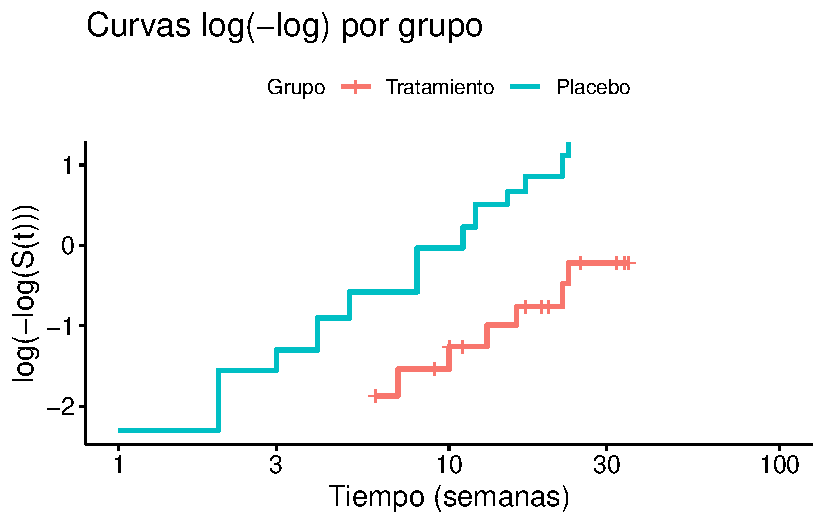
\includegraphics[keepaspectratio]{Unidad4_files/figure-pdf/unnamed-chunk-14-1.pdf}}

\begin{itemize}
\tightlist
\item
  Si las curvas \textbf{son aproximadamente paralelas}, la suposición PH
  se considera razonable.
\item
  Si \textbf{se cruzan} o divergen significativamente, puede haber
  violación.
\end{itemize}

\begin{center}\rule{0.5\linewidth}{0.5pt}\end{center}

\subsection{Residuos de Schoenfeld}\label{residuos-de-schoenfeld}

\begin{itemize}
\tightlist
\item
  Son residuos calculados \textbf{solo en los tiempos de evento}.
\item
  Se usan para evaluar si el \textbf{efecto de una covariable es
  constante en el tiempo} (suposición de riesgos proporcionales).
\end{itemize}

\textbf{Definición:}

\[
\text{Residuo de Schoenfeld} = X_{\text{observado}} - \mathbb{E}[X \mid \text{riesgo}]
\]

\begin{itemize}
\tightlist
\item
  Donde \(X\) es una covariable.
\item
  Se calcula en cada tiempo de evento.
\end{itemize}

\textbf{Interpretación gráfica}

\begin{itemize}
\tightlist
\item
  Los residuos se grafican contra el tiempo.
\item
  Se ajusta una curva de suavizado (por ejemplo, LOESS):

  \begin{itemize}
  \tightlist
  \item
    Si la curva es \textbf{horizontal}, el efecto de la covariable es
    constante.
  \item
    Si tiene \textbf{pendiente creciente o decreciente}, sugiere que el
    efecto \textbf{cambia con el tiempo} → \textbf{violación de la
    suposición PH}.
  \end{itemize}
\end{itemize}

\textbf{Ejemplo de interpretación:}

\begin{itemize}
\tightlist
\item
  Línea plana: suposición PH razonable
\item
  Tendencia ascendente: el efecto crece con el tiempo
\item
  Tendencia descendente: el efecto decrece con el tiempo
\end{itemize}

\begin{center}\rule{0.5\linewidth}{0.5pt}\end{center}

\subsection{\texorpdfstring{Test global de PH con
\texttt{cox.zph()}}{Test global de PH con cox.zph()}}\label{test-global-de-ph-con-cox.zph}

\subsection{¿Qué evalúa?}\label{quuxe9-evaluxfaa}

\begin{itemize}
\tightlist
\item
  Contrasta la \textbf{hipótesis nula} de que el efecto de cada
  covariable es constante en el tiempo.
\item
  Evalúa la \textbf{proporcionalidad de riesgos} para cada covariable y
  de forma global.
\end{itemize}

\textbf{Hipótesis:}

\begin{itemize}
\tightlist
\item
  \(H_0\): la covariable cumple la suposición PH (efecto constante en el
  tiempo)
\item
  \(H_1\): el efecto varía con el tiempo
\end{itemize}

Un \textbf{p-valor bajo (\textless{} 0.05)} indica que \textbf{se viola}
la suposición PH para esa covariable o globalmente.

\subsection{Ejemplo en R}\label{ejemplo-en-r}

\begin{Shaded}
\begin{Highlighting}[]
\NormalTok{test\_ph }\OtherTok{\textless{}{-}} \FunctionTok{cox.zph}\NormalTok{(cox\_model)}
\NormalTok{test\_ph}
\end{Highlighting}
\end{Shaded}

\begin{verbatim}
                 chisq df    p
factor(group) 8.27e-05  1 0.99
logWBC        4.00e-02  1 0.84
GLOBAL        4.02e-02  2 0.98
\end{verbatim}

Esto muestra una tabla con:

\begin{itemize}
\tightlist
\item
  Una fila por covariable y una para el test global
\item
  Estadístico chi-cuadrado y p-valor asociado
\end{itemize}

\textbf{Interpretación}:

\begin{itemize}
\tightlist
\item
  Si el test global es significativo, el modelo \textbf{no cumple} con
  PH en general.
\item
  Si solo una covariable tiene p \textless{} 0.05, considerar
  transformaciones o modelos extendidos.
\end{itemize}

\begin{center}\rule{0.5\linewidth}{0.5pt}\end{center}

\section{Soluciones a Violaciones de
PH}\label{soluciones-a-violaciones-de-ph}

\begin{itemize}
\tightlist
\item
  \textbf{Modelo estratificado}:

  \begin{itemize}
  \tightlist
  \item
    \(h_0(t)\) específico por estrato.
  \end{itemize}
\item
  \textbf{Modelo extendido}:

  \begin{itemize}
  \tightlist
  \item
    Términos dependientes del tiempo.
  \end{itemize}
\end{itemize}

\begin{center}\rule{0.5\linewidth}{0.5pt}\end{center}

\section{Conclusiones}\label{conclusiones}

\begin{itemize}
\tightlist
\item
  Modelo robusto y versátil.
\item
  Permite ajustar múltiples covariables.
\item
  Ideal para datos censurados.
\item
  Evaluar la suposición PH es crucial.
\end{itemize}

\section{Referencias}\label{referencias}

\phantomsection\label{refs}
\begin{CSLReferences}{1}{0}
\bibitem[\citeproctext]{ref-Freireich1963}
Freireich, E. J., Karon, M., Frei, E., Holland, J. F., Taylor, R.,
Hananian, J., Selawry, O., Hoogstraten, B., Wolman, I. J., Abir, E.,
Sawitsky, A., Lee, S., Mills, S. D., Burgert, E. O. J., Spurr, C. L.,
Patterson, R. B., Ebaugh, F. G., James, G. W., \& Moon, J. H. (1963).
The effect of 6‑mercaptopurine on the duration of steroid‑induced
remissions in acute leukemia: A model for evaluation of antileukemic
agents. \emph{Blood}, \emph{21}(6), 699--716.

\bibitem[\citeproctext]{ref-klein2003}
Klein, J. P., \& Moeschberger, M. L. (2003). \emph{Survival analysis:
Techniques for censored and truncated data} (2nd ed.). Springer.

\end{CSLReferences}




\end{document}
